%%==================================================
%% chapter02.tex for SJTU Master Thesis
%% based on CASthesis
%% modified by wei.jianwen@gmail.com
%% Encoding: UTF-8
%%==================================================

\chapter{背景介绍}
\label{chap:background}

本章简要描述了x86架构上系统虚拟化技术的演化历程,并对后文Secure KVM系统和FlexCore系统中涉及到的x86硬件辅助虚拟化技术进行了详细介绍。

\section{x86系统虚拟化技术的演化}

系统虚拟化毫无疑问是推动当前火热云计算大潮的关键技术之一。随着x86处理器凭借着高速增长的处理能力和相对低廉的价格逐渐获得市场的广泛认可,x86平台上的系统虚拟化技术在近20年内取得了长足发展,学术界和工业界中都涌现出了一批富有影响力的系统虚拟化产品,如Bochs、Qemu、Xen、VMware、KVM等。

系统虚拟化是一种资源管理技术,其对真实计算机上的处理器资源、内存资源、存储资源等进行分割并赋予虚拟机,让这些用软件实现抽象出来的虚拟机可以像真实机器一样运行程序。然而,x86处理器的设计初衷并没有囊括系统虚拟化在内,当时在大型主机上普遍适用的``陷入并模拟''(Trap-and-Emulate)虚拟化策略在x86体系结构上未能奏效。这是因为如果按照``陷入并模拟''策略让x86虚拟机以较低权限级别运行,某些敏感x86指令会默默地执行失败而不会产生到虚拟机监控器的陷入,即为虚拟化漏洞,例如POPF指令在Ring 3权限级别执行时不会对\%EFLAGS寄存器系统状态位产生影响也不会触发处理器异常,这便让虚拟机监控器失去了模拟这些敏感指令行为的机会。而Intel出于x86平台的向后兼容性考虑,不可能去改变已发布x86指令集的行为,这个困境在很长一段时间里阻碍了x86平台系统虚拟化的发展。

虽然存在不小的困境,但x86平台上的系统虚拟化还不至于无路可循。一种简单粗暴的解决方法便是``模拟执行''。具体而言,便是分配一个足够大的数组当做虚拟机的内存,根据x86指令集规范,编写一个包含众多case分支的switch语句,获取当前要执行的指令,严格遵照指令集规范说明模拟执行。以上``模拟执行''的方法固然可行,但效率不敢恭维,这种虚拟机至少要比真实机器慢上一个数量级,造成其应用范围非常有限。此外,所谓的动态类型语言,如Python、PHP、Ruby,在被编译成中间代码后,大多也是遵循了这种``模拟执行''的方法,因此执行速度相比于编译型语言快不起来。著名的x86模拟器Bochs便是采用了这种``模拟执行''方法,虽然速度慢,但是兼容性良好,而且不容易出现安全漏洞。

除了``模拟执行'',二进制翻译技术也能用于解决x86平台上的系统虚拟化困境,且具备性能上的优势。如今Java、.NET、JavaScript等语言使用的JIT(Just-In-Time)技术也都属于类似的套路。不能因为指令翻译难实现就因噎废食,一个运行上亿次的for循环,其中如果都是加减之类的数学运算操作,翻译成机器码在处理器上直接执行,肯定比``模拟执行''要快得多。应用到系统虚拟化领域时,在二进制翻译前面,要加上``动态''两字,也就是在虚拟机执行过程中,碰到能翻译的普通指令区块就翻译成目标架构的机器码直接执行,并缓存起来以便后续重复执行,碰到不能直接翻译的特殊指令区块(某些关乎处理器全局状态的敏感指令,例如更改页表地址寄存器值的MOV \%CR3指令)就陷入到虚拟机监控器中或调用虚拟机监控器提供的接口,让虚拟机监控器模拟执行敏感指令,接着再继续对后面的虚拟机代码进行翻译。

VMware的工程师们在1998年首先实现了基于动态二进制翻译(Dynamic Binary Translation)的虚拟机监控器,成功在x86平台上高效实现了系统虚拟化,并推出了VMware Workstation、VMware ESX等商业化产品。Fabrice Bellard完成的Qemu实现原理与上述类似,不过Qemu还支持在x86平台上模拟ARM、MIPS、SPARC、PowerPC等多种处理器架构。VMware针对动态二进制翻译还额外提出了众多其他功能和细节上的优化,这使得其商业化产品性能良好。VMware在x86系统虚拟化领域的创举,也复苏了研究人员和硬件厂商重新发掘这个领域的热情。

动态二进制翻译虽然已经比``模拟执行''快了许多,但由于为了让每条敏感指令得到模拟执行,执行流都要往虚拟机监控器绕一圈(而事实上在大多数情况下,虚拟机内执行多条敏感指令仅仅是为了完成某个单一目的,如在使用了PAE分页机制的32位操作系统中修改某一页表项需要两条MOV指令),这使得虚拟机离真实机器的性能仍然有一定差距。为了提升虚拟机的运行性能,研究人员想到了让虚拟机操作系统辅助配合,即为所谓的``半虚拟化''(Para-virtualization)。``Para''前缀是``with''、``alongside''的意思,也就是说虚拟机与虚拟机监控器不再是严格的上下级关系,而是互信合作的关系。虚拟机操作系统知道自己正处在虚拟化层之上运行,虚拟化层也要在一定程度上信任虚拟机操作系统。Xen在初始阶段便是一个只支持半虚拟化的虚拟化平台,但它为x86系统虚拟化领域开启了新的篇章。

既然动态二进制翻译的难点和性能瓶颈在于模拟执行那些各式各样的敏感指令,我们能不能修改虚拟机的操作系统内核,把那些敏感指令改得``好看''一些,即对虚拟化更友好?以上便是半虚拟化技术的核心思想。毕竟在大多数情况下,我们并不需要对虚拟机刻意``隐瞒'' 虚拟化层的存在,而是要在虚拟机之间提供必要的隔离,同时又不至于造成太多的性能开销。

采用半虚拟化的虚拟机操作系统内核需要经过特殊修改,将原先由敏感指令构成的操作改为对虚拟化层功能接口的调用,即超调用(Hypercall)。在现代操作系统中,由于这些特定体系结构相关的敏感操作实现都被封装起来了(例如Linux内核源码树中的arch/目录),对比动态二进制翻译需要考虑到各种边界情况,半虚拟化对虚拟机操作系统内核源码的修改就显得要简单一些了。相比于使用了动态二进制翻译的全虚拟化(Full-virtualization),半虚拟化是牺牲了通用性来换取性能,因为任何操作系统都可以无修改地运行在全虚拟化平台上,而每个半虚拟化的操作系统内核都要经过人工仔细修改,且要以能获取其源码为前提。

同样的功能,依靠专用硬件实现几乎总是比软件实现性能更好,这几乎已经成为了一条金科玉律。为了顺应市场对于高性能x86系统虚拟化的强烈愿求,Intel和AMD在2005年末几乎于相同的时间推出了x86硬件辅助虚拟化(Hardware-assisted Virtualization)解决方案,并在之后的发展历程中不断对其进行了增强。Intel的解决方案叫做Intel VT(Intel Virtualization Technology)或VMX(Virtual Machine Extension),AMD的解决方案被称为SVM(Secure Virtual Machine)。

在硬件上帮助软件系统实现以前难以完美解决的方案并不是一个新概念。早在1974年,Popek和Goldberg便在``Formal requirements for virtualizable third generation architectures''著名论文中提及了可虚拟化体系结构必须满足的三个必要条件:1)虚拟机监控器提供与真实机器一模一样的虚拟环境;2)运行在虚拟机里的程序在最坏情况下也比物理机慢得不多;3)虚拟机监控器能够完全控制所有的系统资源;3a)虚拟机里的程序不能访问未分配给它的资源,3b)在某些情况下,虚拟机监控器能够回收已经分配给虚拟机的资源。早期的x86指令架构不满足上述条件,因而需要虚拟机监控器进行复杂的动态二进制翻译。既然动态二进制翻译的主要工作在于捕获虚拟机执行中的敏感指令,硬件辅助虚拟化中处理器最重要的职责便是捕获这些关键事件并将其交由虚拟机监控器处理。

为了维持对早期x86程序的兼容性,硬件辅助虚拟化在x86体系结构原有的四个执行特权级(Ring)基础上,增加了一个专供虚拟机监控器使用的与原先特权级别正交的根模式(Root mode),而虚拟机中的操作系统和应用程序则处于独立的非根模式(Non-root mode)运行。这样一来,尽管虚拟机操作系统运行在Ring 0,其执行敏感指令时仍然会触发异常并被处理器自动捕获,从而陷入到位于根模式的虚拟机监控器中,待到虚拟机监控器完成处理后再使用VMLAUNCH或VMRESUME指令让执行流返回虚拟机。

下一节将对硬件辅助虚拟化技术进行详细阐述。

\section{硬件辅助虚拟化技术}

\subsection{概述}

硬件辅助虚拟化技术,顾名思义,就是在处理器、芯片组和I/O设备等硬件层面上加入专门针对虚拟化的支持,让虚拟机监控器能够更容易、高效率地实现系统虚拟化。

之所以要在硬件层面给予辅助,原因来自多方面。首先,由于原先x86体系结构存在虚拟化漏洞,单纯的``陷入并模拟''方案是行不通的,而动态二进制翻译技术难以处理虚拟机内的自修改代码和自参考代码,采用半虚拟化技术的前提是能够获取虚拟机内操作系统的源码;其次,由于硬件特性的限制,某些虚拟化功能尽管理论上可以用软件方法实现,但是实现途径异常曲折复杂,一个典型的例子便是限制虚拟机访存的影子页表(Shadow Page Table,SPT),其受限于原先处理器硬件只能提供一层内存地址转化功能;最后,某些使用软件方法实现的虚拟化功能往往性能和隔离性达不到要求,例如网卡磁盘等I/O设备的虚拟化。以上提及的这些问题,只有在处理器、芯片组等硬件层面上提供相应的辅助支持,才能得以完全解决。

两大处理器厂商Intel和AMD都想方设法在系统虚拟化领域中占得先机,但是AMD的虚拟化技术在时间上要比Intel落后几个月。Intel自2005年末开始便在其处理器产品线中推广应用Intel VT(Intel Virtualization Technology)硬件辅助虚拟化技术。

AMD处理器提供的硬件辅助虚拟化技术虽然与Intel VT在细节上存在差异,不过它们的主体架构和核心思想是类似的,下文章节将以Intel VT为例详细介绍硬件辅助虚拟化技术。

\subsection{CPU虚拟化}

Intel VT在x86处理器原有的四个运行权限级别基础上,引入了两种新的操作模式,统称为VMX操作模式。

\begin{itemize}
\item VMX根模式(VMX Root Mode):虚拟机监控器所处的运行模式,基本等同于加入硬件辅助虚拟化支持以前的处理器工作模式,以下简称根模式。
\item VMX非根模式(VMX Non-Root Mode):客户虚拟机所处的运行模式,虚拟机中的二进制代码无需经过特殊处理直接以该模式在处理器硬件上直接运行,以下简称非根模式。
\end{itemize}

这两种VMX操作模式与32位x86处理器原有的Ring 0$\sim$Ring 3权限级别是正交的,即在每种VMX操作模式下都有Ring 0$\sim$Ring 3这四个运行权限级别。Intel VT采用这种改动方式的理由很明显,x86体系结构不能借助``陷入并模拟''这种经典方式进行系统虚拟化的根本原因在于其中的19条指令无法在低权限级别产生陷入,从而导致了虚拟化漏洞。如果简单地修改这19条指令的语义,让其在低权限级别运行时也能产生陷入,便会破坏与之前软件代码的二进制兼容性,而这是不可接受的。通过引入新的处理器运行模式,并重新定义敏感指令(包括之前的19条指令)在非根模式下的运行行为,即让其在非根模式运行时也能够产生到根模式的陷入,便能很好地填补先前的虚拟化漏洞。同时,Intel VT保持了x86原先所有指令在根模式下的运行语义不变,因此之前的二进制代码仍能正常运行。Intel VT通过这种途径很好地解决了x86系统虚拟化问题。

虚拟机在支持Intel VT技术的x86处理器上运行过程如下:

\begin{figure}[!htp]
  \centering
  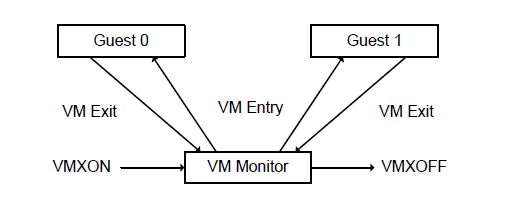
\includegraphics[width=0.7\textwidth]{chap2/mode.png}
  \bicaption[fig:mode]{Intel VT支持下的虚拟机的运行循环}{Intel VT支持下的虚拟机的运行循环}{Fig}{Virtual machine life cycle with Intel VT}
\end{figure}

\begin{enumerate}
\item 虚拟机监控器执行VMXON指令让处理器进入VMX根模式,为运行客户虚拟机做准备。
\item 虚拟机监控器执行VMLAUNCH或者VMRESUME指令产生VM Entry,执行流转移至虚拟机内部的代码,处理器处于VMX非根模式运行。
\item 由于客户虚拟机执行了敏感指令,或者在其运行期间发生了硬件中断或软件异常,VM Exit被触发,执行流重新回到虚拟机监控器,处理器回到VMX根模式运行。
\item 虚拟机监控器根据虚拟化陷入发生的原因进行相应的处理,处理完成后,虚拟机监控器可以选择继续回到先前运行的客户虚拟机或者重新挑选另一个客户虚拟机运行,即回到步骤2。
\item 所有的客户虚拟机运行完毕,虚拟机监控器使用VMXOFF指令让处理器从VMX根模式退出。
\end{enumerate}

可以看到,虚拟机的顺利运行,就是一个在虚拟机监控器->虚拟机->虚拟机监控器->虚拟机->$\cdots$间不断循环的过程。以上流程中包含了两个处理器在VMX根模式和VMX非根模式间切换的行为,分别为从根模式切换到非根模式的VM Entry和从非根模式切换到根模式的VM Exit。

\begin{enumerate}
\item VM Entry:虚拟机监控器在VMCS中设置好虚拟机接下来运行的上下文环境,使用VMLAUNCH(用于第一次或刚执行VMCLEAR后的VM Entry)或VMRESUME(用于执行过VMLAUNCH虚拟机的后续VM Entry)使处理器由根模式向非根模式转换,转换完成后,虚拟机内部的代码开始在处理器上直接执行。
\item VM Exit:由于某些原因,如虚拟机执行了敏感指令或发生了外部中断,处理器暂停执行虚拟机内部代码,从非根模式回退至根模式。虚拟机监控器会根据VM Exit发生的具体原因,对应地给予处理,如模拟指令行为等。在硬件辅助虚拟化中,处理VM Exit是虚拟机监控器最主要的职责。
\end{enumerate}

VMCS(Virtual Machine Control Structure)被用于在虚拟机监控器和处理器硬件之间共享虚拟机执行的上下文环境和交换数据信息。虚拟机监控器可以通过修改VMCS中的某些位域来控制虚拟机在非根模式下的运行行为,在VM Exit发生时虚拟机监控器可以从VMCS中获取陷入发生的具体原因,此外虚拟机某些关键寄存器的值在VM Exit和VM Entry发生时会在VMCS中进行保存和恢复。VMCS占用一个对齐的4KB大小的内存区域,即一个普通内存页框,其中主要的结构组成如下:

\begin{enumerate}
\item 客户虚拟机状态域,包括虚拟机部分关键寄存器的值、虚拟处理器可中断状态。
\item 宿主机状态域,主要是宿主机部分关键寄存器的值。
\item 虚拟机执行控制域,控制客户虚拟机在非根模式下的执行行为。
\item 虚拟化陷入控制域,控制虚拟化陷入的产生条件。
\item 虚拟机进入控制域,控制处理器从根模式向非根模式转换
\item 虚拟化陷入信息域,记录了虚拟化陷入发生的具体原因,其值由硬件自动更新。
\end{enumerate}

Intel为了在处理器上支持硬件辅助虚拟化,扩展了原有的x86指令集,增添了13条新指令,列举如下。其中,除去VMCALL和VMFUNC被用于虚拟机内部在非根模式下执行,其余的11条指令适用于在处理器根模式下执行。

\begin{enumerate}
\item INVEPT:使EPT中的特定内存地址翻译失效。
\item INVVPID:使与VPID对应的某虚拟机所有的内存地址翻译失效。
\item VMCALL/VMFUNC:发起向虚拟机监控器的请求调用。
\item VMCLEAR:将VMCS数据强制由处理器刷新回内存。
\item VMLAUNCH/VMRESUME:启动或唤醒虚拟机。
\item VMPTRLD/VMPTRST:加载或存储指向VMCS的内存地址。
\item VMREAD/VMWRITE:读取或写入当前加载VMCS的某些位域。
\item VMXON/VMXOFF:使处理器进入或离开VMX操作模式。
\end{enumerate}

\subsection{内存虚拟化}

在虚拟化环境中,存在着两层内存地址转换关系,即从客户虚拟机虚拟地址到客户虚拟机物理地址的第一层转换,和从客户虚拟机物理地址到宿主机物理地址的第二层转换。而在原先的x86处理器上,硬件只提供一层地址转换,即通过\%CR3寄存器指向的页表实现虚拟地址到物理地址的转换。因此,在以动态二进制翻译等技术软件实现的虚拟化平台上,虚拟机监控器需要为虚拟机内部的每一份页表对应维护一份影子页表(对于Linux,虚拟机监控器要为其中的每个进程维护一份影子页表,并在虚拟机内部发生进程切换时对应切换影子页表),此维护过程需要监视虚拟机内部对于页表的修改且要仔细处理可能发生的各种边界情况,增大了虚拟机监控器的设计实现难度,且会对虚拟机性能造成较大影响。

Intel在2007推出的第二代硬件辅助虚拟化技术中增添了对于扩展页表(Extended Page Table,EPT)特性的支持,直接在处理器硬件上支持两层内存地址转换,大大降低了内存虚拟化的实现难度,同时也提升了虚拟机的运行性能。

EPT表的大体结构与普通x86页表类似,都采用多级结构,其中每个EPT页表项的高位部分用于记录页框号,低12位则用于记录一些标志位(是否可读、是否可写、是否可执行、是否是超页)。VMCS中有专门的位域用于设置EPT表,虚拟机中代码的访存范围受到EPT表的限制。

\begin{figure}[!htp]
  \centering
  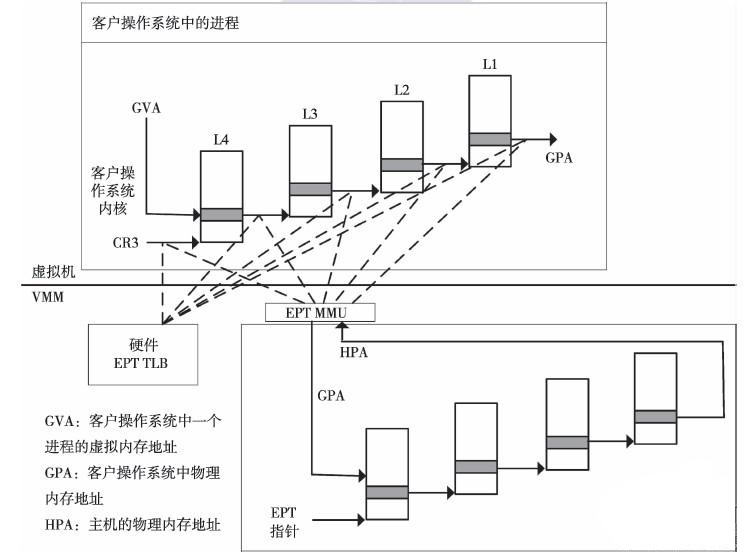
\includegraphics[width=0.7\textwidth]{chap2/ept.png}
  \bicaption[fig:ept]{EPT表内存地址翻译示意}{EPT表内存地址翻译示意}{Fig}{Illustration on memory address translation of EPT}
\end{figure}

此处假设客户虚拟机中的普通页表和EPT表都是4级结构,处理器完成一次完整内存地址转换的流程如下。处理器首先根据虚拟机内\%CR3寄存器值获得L4页表地址,此L4页表地址为客户虚拟机物理地址(Guest Physical Address,GPA),因此处理器还要参考EPT表来实现该GPA到宿主机物理地址(Host Physical Address,HPA)的转换。处理器会先到TLB中进行查找,如果其中没有对应的缓存项,处理器再退而求其次到EPT表中逐级进行查找,如果仍没有找到,处理器则会抛出EPT页故障并交由虚拟机监控器处理。获得L4页表的HPA后,处理器根据待翻译地址偏移和L4页表内容,来确定L3页表的GPA,之后再通过查找EPT表获取L3页表的HPA。按照类似的步骤,处理器依次访问L2和L1页表,获得待翻译地址对应的GPA,最后再通过EPT表转换为HPA,并将该映射关系在TLB中缓存。在以上内存地址翻译流程中,若是处于最不利情况即TLB为空时,处理器需要经历共计24(5*4+4)次访存,不过在之后TLB缓存生效情况下,虚拟机内的访存速度与非虚拟化环境下无异。为了提升虚拟机内的访存效率,处理器通过增大TLB容量来减少地址翻译过程中的TLB缺失率。

\subsection{中断虚拟化}

虚拟机的运行离不开众多的I/O设备,例如磁盘和网卡,这些I/O设备一般都是由虚拟机监控器或专门的用户态程序如Qemu来进行模拟,而这些I/O设备的模拟离不开中断虚拟化。

在虚拟化环境中,虚拟机监控器为客户虚拟机维护了一套与真实物理机器上中断架构类似的虚拟中断架构,其中包括了虚拟PIC、虚拟Local APIC、虚拟I/O APIC等软件实体。当虚拟设备需要发送中断时,虚拟设备会调用虚拟I/O APIC提供的接口发送中断。虚拟I/O APIC根据中断具体情况,将中断路由至对应的虚拟Local APIC。虚拟Local APIC再进一步调用Intel VT中的事件注入机制将中断注入到对应的虚拟处理器。

\section{本章小结}

本章对论文中所涉及到的一些相关背景知识进行了介绍。本章在一开始先简要叙述了x86体系结构上系统虚拟化的发展历程,然后从CPU虚拟化、内存虚拟化和中断虚拟化三个方面着重介绍了x86上的硬件辅助虚拟化技术,为以后的章节做了铺垫。